%\documentclass{standalone}

%\usepackage{mathpazo}
%\usepackage{tikz}

\usetikzlibrary{calc}
\usetikzlibrary{positioning}
\usetikzlibrary{shapes}

%\begin{document}

\tikzstyle{box} = [rectangle, rounded corners, draw=black, text width=10em, minimum height=3em, text centered]
\begin{figure}[H]
  \centering
  \footnotesize
  %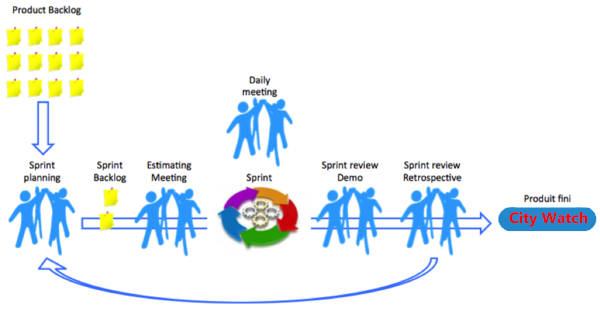
\includegraphics[width=\textwidth]{./figures/scrum-model.tex}
\begin{tikzpicture}

  \node[box]
    (sprints) {Sprints};
  \node[box, left=4em of sprints]
    (planning) {Planning \& System Architecture};
  \node[box, right=4em of sprints]
    (closure) {Closure};

  \draw[->,latex-,line width=0.1em] (5:6em) arc (5:85:6em) node[right=2em] {Wrap};
  \draw[->,latex-,line width=0.1em] (95:6em) node[left=2.5em] {Develop} arc (95:175:6em);
  \draw[->,latex-,line width=0.1em] (185:6em) arc (185:265:6em) node[left=2em] {Adjust};
  \draw[->,latex-,line width=0.1em] (275:6em) node[right=2.5em] {Review} arc (275:355:6em);

  \draw[->,latex-] (planning.west) -- +(-2em,0);
  \draw[->,-latex] (planning.east) to (sprints.west);
  \draw[->,-latex] (sprints.east) to (closure.west);
  \draw[->,-latex] (closure.east) -- +(2em,0);

\end{tikzpicture}
\caption[Méthode Scrum]{La méthode Génie Logiciel Scrum comme décrite par \textcite{Schwaber1995}.}
\captionsource{Daniel G. Siegel, Typical Development Processes of Free and Open Source Software Projects}
\label{fig:scrum-model}
\end{figure}

%\end{document}
